\subsection{Visualizzazione dei Dati di Monitoraggio}\label{VisualDati}

L'utente, una volta che si trova nella sezione del plug-in dedicata alla visualizzazione dei monitoraggi attivi (a cui ha accesso mediante l'operazione descritta in §\ref{MonitoraggiAttivi}), può visualizzare gli effettivi dati di monitoraggio provenienti da una qualsiasi delle reti in fase di monitoraggio.\\
Nello specifico l'utente può selezionare da un menù a tendina (Figura \ref{SelezioneMonitoraggio}) la rete, tra quelle al momento in fase di monitoraggio, di cui desidera visualizzare i dati.

\begin{figure}[H]
	\begin{center}
		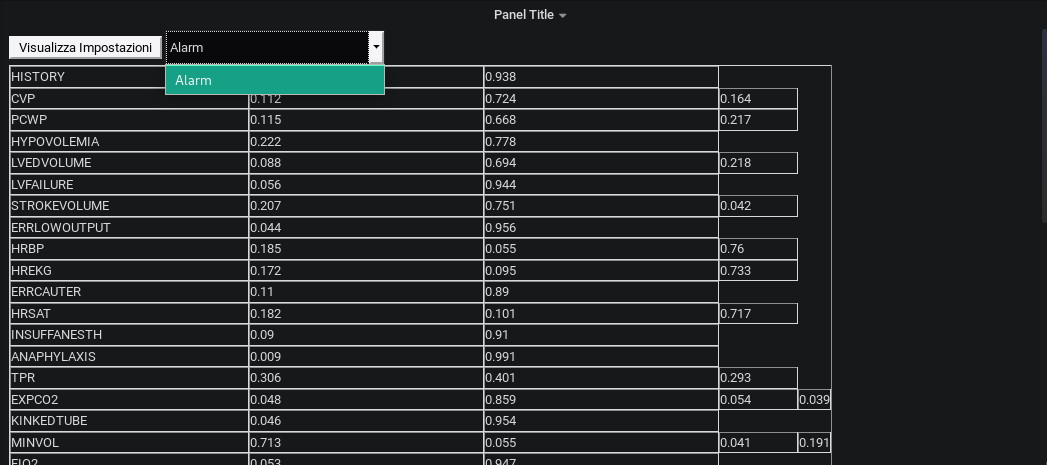
\includegraphics[scale=0.6]{./images/SelezioneMonitoraggio.png}
		 \caption{Menù a Tendina per la Selezione della Rete di cui Visualizzare i Dati di Monitoraggio}	
		 \label{SelezioneMonitoraggio}
	\end{center}
\end{figure}

Una volta selezionata la rete l'utente riceve periodicamente i dati di monitoraggio aggiornati (Figura \ref{DatiMonitoraggio}).\\
Tali dati sono rappresentati sotto forma di una misura di probabilità, associata ad ogni stato di ogni nodo della rete. Tali probabilità vengono aggiornate ciclicamente in base a quanto definito dall'utente in sede di configurazione della politica temporale di ricalcolo (§\ref{policy}).

\begin{figure}[H]
	\begin{center}
		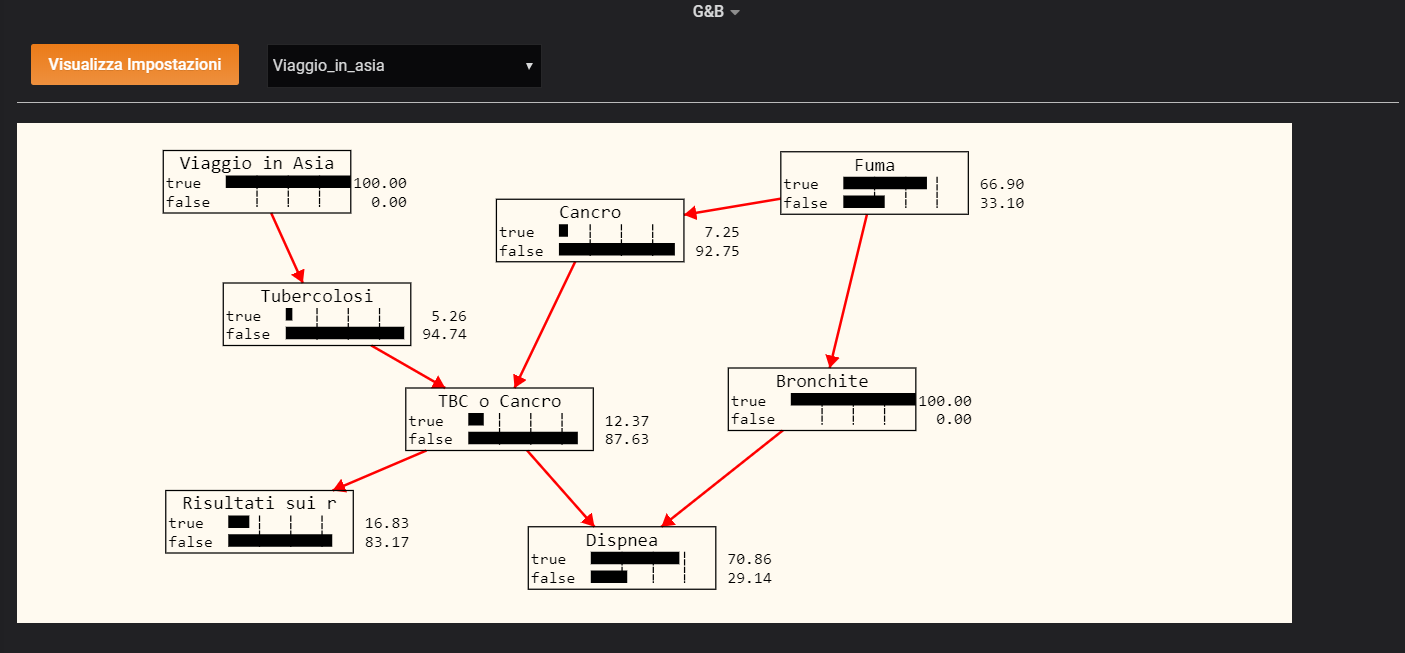
\includegraphics[scale=0.5]{./images/DatiMonitoraggio.png}
		 \caption{Visualizzazione dei dati di Monitoraggio}	
		 \label{DatiMonitoraggio}
	\end{center}
\end{figure}
